%
% $Id: blank.tex,v 2.0 2010-01-05 18:50:50+09 kobayasi Exp $
%
% Mar 21, 2001:  Revision Control Started!!
%
\documentclass[11pt]{jarticle}
\usepackage{newcent}             % PDFへの変換後の品質を高める
\usepackage[dvipdfmx]{graphicx}
\usepackage{wrapfig} % 文章を図に回り込ませて配置するもの
\usepackage{comment} % 複数行をコメントアウトするためのもの
\usepackage{color}
\definecolor{purple}{rgb}{0.6,0,0.4}
\definecolor{brown}{cmyk}{0,0.81,1,0.60}
\usepackage{listings, jlisting}
\renewcommand{\lstlistingname}{ソース}
\lstset
{
breaklines = true,
language=Java,
keywordstyle={\color{purple}},
commentstyle={\color{brown}},
numbers=left,
frame=single,
tabsize=4
}


%
%\usepackage[doctor]{gaiyo}      % 博士論文要旨の場合
%\usepackage[master]{gaiyo}      % 修士論文要旨の場合
\usepackage[senior]{gaiyo}               % 卒業研究概要の場合
% \usepackage[junior]{gaiyo}      % 専門演習レポートの場合

\title{スマートフォンのモーションセンサを利用した個人認証アプリケーションの開発}
\id{情11-0170}
\author{高坂 賢佑}
\teacher{小林 孝史}

\begin{document}
\maketitle

\section{はじめに}
スマートフォンが徐々に普及しつつある現在,スマートフォンの個人認証方法は画面上に表示されるソフトウェアキーボードのテンキーを用いたパスコード認証が大部分を占めている.
しかし,この認証方法は画面ロックを解除するたびに画面に表示されたソフトウェアキーボードを目で見て指でタッチして操作する必要があるため,ユーザにとっては煩雑な作業である.
また,パスコード認証では,あらかじめ決められた文字種の中から1つずつ選択したものを元にパスコードを構築していくという性質上,パターン数が限られ,自由度が限定されてしまう.

そこで,パスコード認証が抱える認証の煩雑さを解消し,かつ,自由度が高くより直感的に個人認証を行えるアプリケーションを開発する.
このアプリケーションには,一般的なスマートフォンに搭載されている加速度センサとジャイロセンサを用いることとする.

\begin{comment}
\section{使用するセンサに関して}
本アプリケーションには,二種類のモーションセンサを利用する.

% センサ座標系を回りこみで図示
\begin{wrapfigure}{r}{60mm}
    \begin{center}
        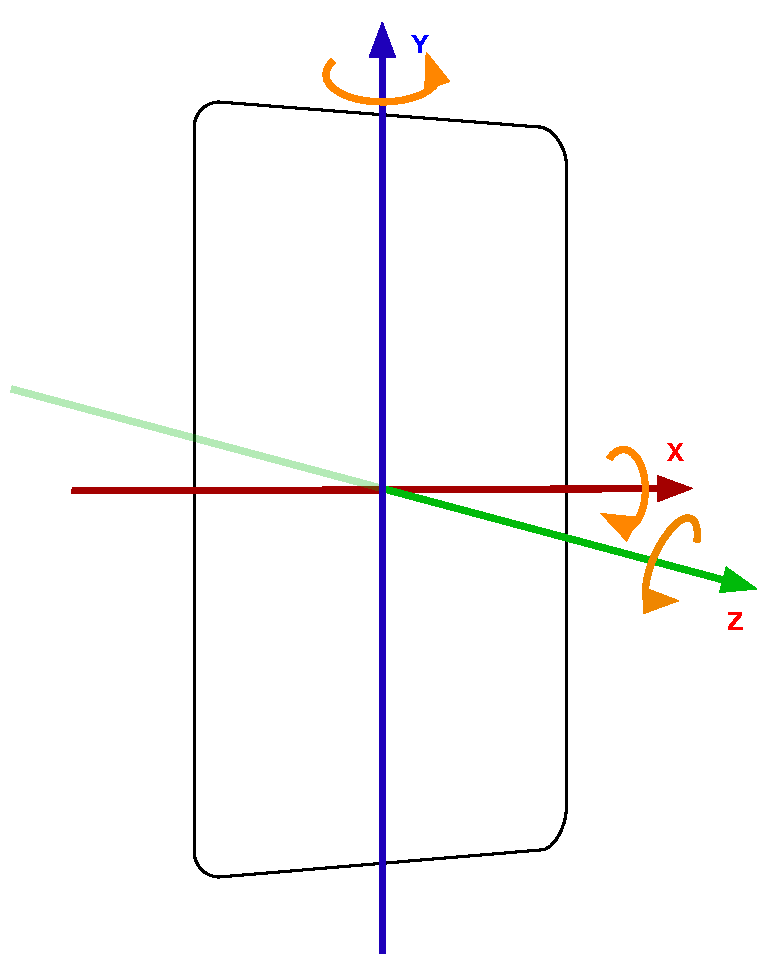
\includegraphics[width=50mm, bb=0 0 373 469]{SmartphoneSensor.pdf}
        \caption{モーションセンサの座標系}
        \label{sensor}
    \end{center}
\end{wrapfigure}

\subsection{加速度センサ}
加速度センサとは,X軸,Y軸,Z軸の基準軸に対して直線運動の加速度をそれぞれ検出し,値として取り出すことの出来るセンサである.
ここでいう加速度とは,端末における単位時間あたりの速度の変化率のことを指し,図\ref{sensor}における直線で示した矢印の方向が正の値,逆が負の値をとる.

\subsection{ジャイロセンサ}
ジャイロセンサとは,X軸,Y軸,Z軸の基準軸に対して回転運動の角速度をそれぞれ検出し,値として取り出すことの出来るセンサである.
ここでいう角速度とは,端末における単位時間あたりの回転角のことを指し,図\ref{sensor}における橙色で示した回転の方向が正の値,逆が負の値をとる.
\end{comment}

\section{本研究のシステム}
本研究では,兎澤の研究\cite{tozawa}で挙げられていた,全体的な認証成功率の低さや対応できるモーションに限りがあるという点を改善することを目標とする.
システムの動作フローを図\ref{flow}に示す.

\begin{wrapfigure}{r}{60mm}
    \begin{center}
        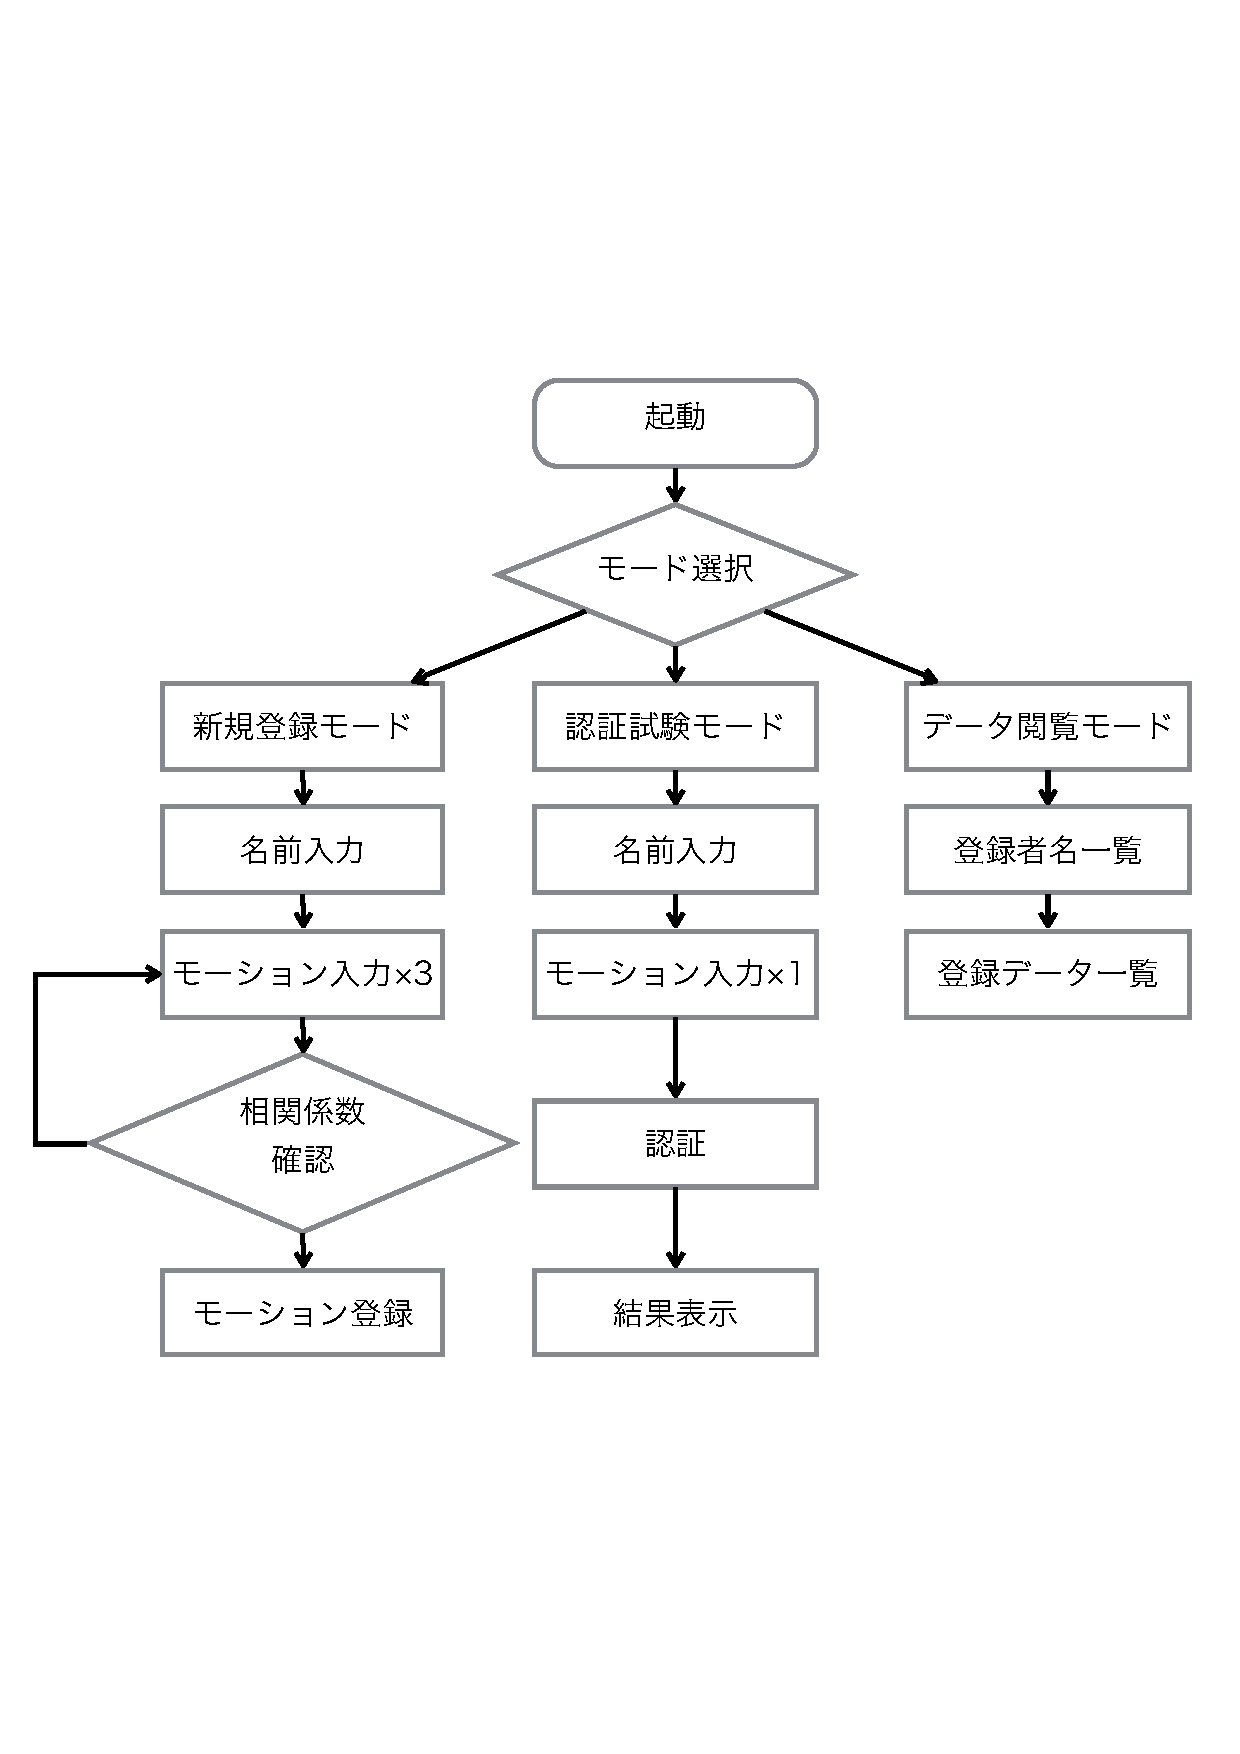
\includegraphics[width=55mm, bb=0 183 594 670]{Flow.pdf}
        \caption{動作フロー図}
        \label{flow}
    \end{center}
\end{wrapfigure}

まずはじめに,アプリケーション起動後に表示されるモード選択ダイアログより,新規登録モードを選択する.
このモードでは,個人認証を行う際の鍵情報となるモーションデータをユーザ名を指定して登録することができる.
モーションの取得は三回行われる.
データ取得完了後,まずは回数ごとのモーションが同一のものであるか確認し,モーション取得時に生じうる時間的なズレを必要に応じて修正する.
修正が終われば,次にモーション取得時の手の細かなブレなどから生じうるデータに対する影響を取り除く,フーリエ変換を用いたローパスフィルタ処理を行う.
そして最後にデータの振れ幅があらかじめ設定した閾値より小さい場合,つまりモーションの動きが小さい場合には,あらかじめ設定した値を用いてデータの増幅処理を行い,これらの処理を終えた三回分のデータの平均値を登録する.

これらの処理を行うことで,先行研究で挙げられていた,認証成功率の低さや対応できるモーションに限りがあるという問題に対応する.

認証試験モードでは,あらかじめ新規登録モードにおいてモーションデータの登録を行ったユーザ名を指定し,そのデータと新たに一回入力したモーションデータとの相関係数を算出し,これで個人認証を行う.

データ閲覧モードでは,新規登録モードにおいて登録したユーザ名およびモーションデータをリスト形式で閲覧する事ができる.

\section{実験と考察}

\section{今後の課題}

 % 参考文献
\begin{thebibliography}{9}
    \bibitem{tozawa}兎澤星伸,”三軸加速度センサ及び三軸ジャイロセンサを用いた認証アプリケーションの開発”,2012年度卒業研究.
\end{thebibliography}

\end{document}
